\chapter{Resultados}
\label{chap:result}
Importante sempre ter um parágrafo introdutório para explicar os resultados encontrados.

% %--------- NEW SECTION ----------------------
% \section{Testes unitários}
% \label{sec:testu}
% \lipsum[1]

% \section{Integração do sistema}
% \label{sec:intsis}
% \lipsum[1]

% %--------- NEW SECTION ----------------------
% \section{Testes integrados}
% \label{sec:testi}
% \lipsum[1]

\section{Diagrama de classes}
\label{sec:class}
O diagrama de classes é uma representação visual das classes do sistema e seus relacionamentos. Ele é utilizado para descrever a estrutura do sistema e como as classes interagem entre si. A Figura \ref{fig:diagrama_classes} apresenta o diagrama de classes do sistema desenvolvido.
\begin{figure} [h!]	
    \centering
    \caption{Meu diagrama de classes}
    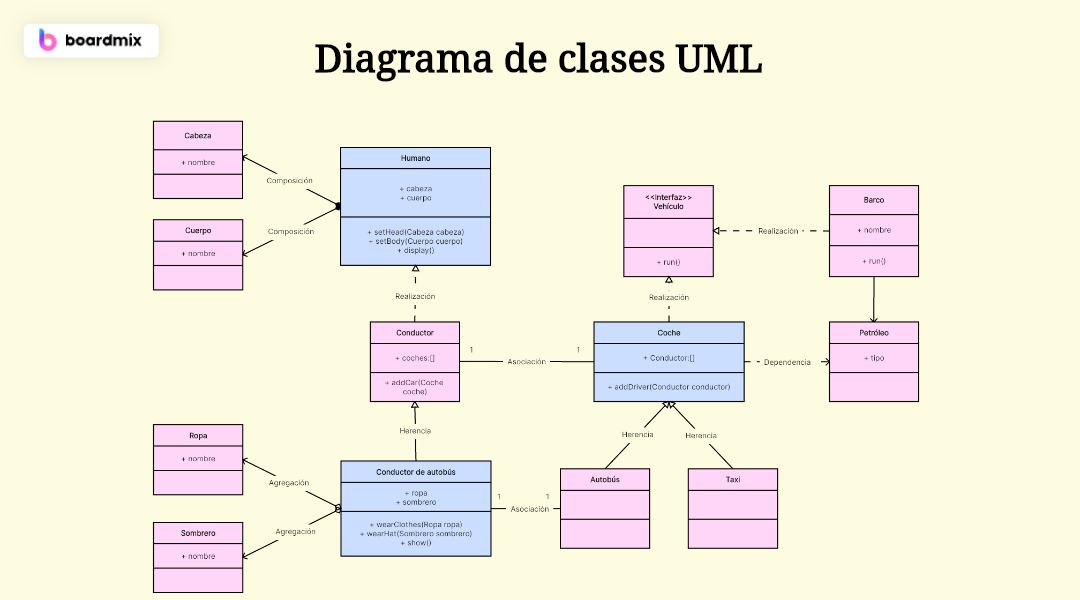
\includegraphics[width=0.8\textwidth]{Figures/diagrama-de-clases-uml.png}
    \caption*{Fonte: Autoria própria.}
    \label{fig:diagrama_classes}
\end{figure}

favor olhar a seção \ref{sec:class}.


\section{Diagrama de casos de uso}
\label{sec:casos}
O diagrama de casos de uso é uma representação visual dos casos de uso do sistema e os atores envolvidos. Ele é utilizado para descrever as funcionalidades do sistema e como os usuários interagem com ele. A Figura \ref{fig:diagrama_casos} apresenta o diagrama de casos de uso do sistema desenvolvido.

\section{Diagrama de sequência}
\label{sec:sequencia}   
O diagrama de sequência é uma representação visual da interação entre os objetos do sistema ao longo do tempo. Ele é utilizado para descrever como os objetos interagem entre si para realizar uma determinada funcionalidade. A Figura \ref{fig:diagrama_sequencia} apresenta o diagrama de sequência do sistema desenvolvido. 








